\section{Elaboración de la recomendación final}
\subsection{Autoevaluación}
\paragraph{}
En esta sección se ha cumplido los objetivos correspondientes al 10
\subsection{Introducción}
\paragraph{}
Tras haber analizado los distintas funcionalidades que nos ofrece Odoo durante tres meses somos capaces de emitir una recomendación clara y fundamentada sobre la viabilidad de implementar Odoo en nuestra empresa UZ-on-Marketing. Este veredicto final es producto de una evaluación objetiva y rigurosa, considerando tanto los aspectos positivos como las limitaciones.
\subsection{Metodología}
\paragraph{}
Tras haber analizado cada uno de las distintas funcionalidades que nos ofrece Odoo; hemos evaluado los módulos que nos ofrece Odoo, hemos analizado las virtudes y defectos de cada uno. Creemos que la mejor forma de realizar la evaluaciones es proporcionando una nota numérica de forma objetiva, basada en ejes de selección y determinar si cada módulo supera un umbral. Por lo tanto, previo a realizar este análisis final hemos tenido que definir cuales son los ejes de selección. Para ello, hemos decidido utilizar un estándar reconocido en la valoración de la adquisición de software. En concreto la \href{https://iso25000.com/index.php/normas-iso-25000/iso-25010}{ISO/IEC 25010}, esta decisión se ha basado en ser su amplio alcance y reconocimiento internacional. Este estándar ofrece un enfoque integral para evaluar la calidad del software en múltiples dimensiones, incluyendo características clave como funcionalidad, usabilidad, eficiencia y seguridad. Su flexibilidad y adaptabilidad lo hacen aplicable a una variedad de tipos de software, asegurando una evaluación precisa y consistente. Además, ISO/IEC 25010 se centra en las necesidades del usuario final, facilitando la comparación entre productos y garantizando la selección del software que mejor se adapte a nuestras necesidades y requisitos específicos. Esta ISO esta compuesta por 9 características de calidad, las cuales a su vez se dividen en más factores. Para realizar el análisis de este ERP hemos hecho una selección. A cada uno de los factores hemos asignado un peso y establecido unos rangos, definiendo si descartamos el software, necesitamos una segunda opición o si lo recomendamos; siendo \textless{} MAX 1/3, entre 1/3 MAX y 2/3 MAX, y \textgreater{} MAX 2/3 respectivamente. Por úlitmo hemos realizado una tabla de agregación de resultados y una conclusión.

\begin{figure}
    \centering
    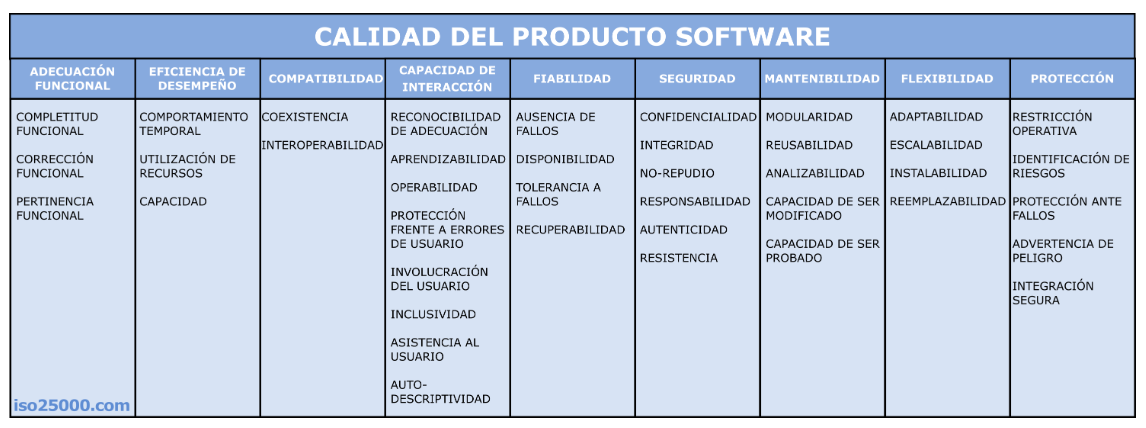
\includegraphics[width=1\linewidth]{final/isoo.png}
    \caption{ISO/IEC 25010}
    \label{fig:enter-label}
\end{figure}
\newpage
\subsection{Resultados y análisis}
\paragraph{}
Para hacer el análsis de Odoo y determinar si debemos adquirir hemos seleccionado 10 factores de la ISO/IEC 25010, como hemos comentado previamente.
Estos son los factores que consideramos más relevantes para Uz-on-Marketing:
\begin{itemize}
    \item \textbf{Corrección funcional}, capacidad del producto o sistema para proveer resultados exactos cuando es usado por los usuarios especificados.
    \item \textbf{Comportamiento temporal}, grado en que un producto realiza sus funciones de forma que el tiempo de respuesta y el ratio de rendimiento cumple los requisitos especificados.
    \item \textbf{Interoperabilidad}, capacidad de dos o más sistemas o componentes para intercambiar información y utilizar la información intercambiada.
    \item \textbf{Aprendizabilidad}, capacidad del producto que permite al usuario aprender su funcionamiento dentro de un tiempo especificado.
    \item \textbf{Operabilidad}, capacidad del producto que permite al usuario operarlo y controlarlo con facilidad.
    \item \textbf{Ausencia de fallos}, capacidad del sistema de llevar a cabo sus funciones sin fallos bajo condiciones normales de operación.
    \item \textbf{Confidencialidad}, capacidad de asegurar que los datos solo son accesibles a aquellos con autorización para ello.
    \item \textbf{Modularidad}, capacidad de un producto para evitar que los cambios en un componente afecten a otros componentes, pero trabajen conjuntamente entre ellos.
    \item \textbf{Instalabilidad}, facilidad con la que el producto se puede instalar y/o desinstalar de forma exitosa en un determinado entorno.
    \item \textbf{Integración segura}, capacidad de un producto para mantener la seguridad durante y después de la integración con uno o varios componentes.
\end{itemize}
\paragraph{}
A cada uno de los factores hemos asignado un peso:
\begin{table}
\centering

\begin{tblr}{
  hlines,
  vlines,
}
\textbf{Factor}                  & \textbf{Peso}  \\
Corrección funcional    & 9     \\
Comportamiento temporal & 4     \\
Interoperabilidad       & 5     \\
Aprendizabilidad        & 10    \\
Ausencia de fallos      & 8     \\
Operabilidad            & 10     \\
Confidencialidad        & 4     \\
Modularidad             & 5     \\
Instalabilidad          & 3     \\
Integración segura      & 2     \\
TOTAL                   & 60   
\end{tblr}
\caption{Tabla de los pesos asignados a cada factor}
\end{table}

\paragraph{}
El peso total obtenido es 60. Y en consecuencia, los rangos establecidos son: 
\begin{itemize}
    \item \textless{} (60*1/3 = 20) =\textgreater{} Descartamos el software
    \item entre (60*1/3 = 20) y (60*2/3 = 40 ) =\textgreater{} Necesitamos una segunda opinión 
    \item \textgreater{} (60*2/3 = 40) =\textgreater{} Recomendamos el software
\end{itemize}
\paragraph{}
Durante estos dos meses hemos estado analizando cada uno de los módulos más relevantes y que se adecuan a nuestras necesidades. Se ha evaluado objetivamente cada uno de los módulos y hemos llegado a las siguientes conclusiones de cada uno de los módulos.

\begin{itemize}
    \item Instalación: Tanto la instalación de Odoo en máquinas locales como en máquinas remotas es sencillo. Requiere ciertos conocimientos intermedios sobre administración de sistemas, sin embargo, no han surgido problemas que hayan dificultado su instalación. Se podría reconsiderar el servidor en el que alojar la máquina remota, según los intereses de la compañía.
    \item Configuración funcional, detalles y organización de la empresa: Módulo fácil de configurar e intuitivo. Es importante que este módulo sea asi dado  su gran relevancia al ser la base en la que se lleva a cabo el resto de funcionalidades.
    \item Configuración funcional, imagen corporativa: Odoo ofrece buenas herramientas para realizar de manera sencilla y con ua gran flexibilidad para adecuarla a las necesidades de cada negocio. La configuración y personalización de la web consideramos que también es una tarea esencial y que toda empresa ha de realizar.
    \item Configuración técnica, copia de seguridad: Realizar copias de seguridad de la base de datos es una tarea que se puede automatizar de forma sencilla siguiendo los pasos descritos. El lugar en el que almacenarlas se podría modificar según las necesidades y recursos de la empresa.
    \item Configuración técnica, correo: Este módulo es fundamental para toda empresa y es necesario que su implementación en Odoo sea rápida y sencilla. Esta funcionalidad permite la comunicación interna y externa, automatizando el envío de correos y ahorrando tiempo y coste a la compañía. Además, existe una muy buena documentación para su configuració por lo que no debería ser díficil de implementar.
    \item Proyectos: Este módulo para nosotros es uno de los mejores que nos proporciona Odoo. Es sencillo de utilizar, intuitivo y muy útil. Nos permite gestionar las tareas de los distintos equipos de trabajo de una forma visual y eficiente. Además tiene un buen nivel de personalización. 
    \item Gestión de producción (MRP): En este apartado se gestiona una funcionalidad que referencia una actividad esencial dentro de la mayoria de empresas. Sin embargo, se han encontrado problemas para realizar la configuración completa de los módulos ya que la automatización de los módulos es una tarea compleja y que requiere una cantidad considerable de tiempo para conseguir su correcto funcionamiento. Por lo tanto, la valoración es negativa. 
    \item Relación con clientes (CRM): La tarea que desempeña este módulo escompleja, pero que se ha podido implementar relativamente rápido ya que a pesar de su gran cantidad de posibilidades a la hora de realizar la configuración es intuitivo.
    \item Gestión de personal (HR): Todo empresa en algun momento va a necesitar gestionar sus empleados, lo que hace que este módulo sea muy importante en la gestión de una empresa. Se ha configurado de forma sencilla. Cabe destacar que pensamos que esta funcionalidad no es muy escalable si el número de empleados aumenta considerablemente.
    \item Contabilidad y finanzas (FICO): Odoo 17.0 tiene un gran problema con este módulo y se tiene que recurrir a software externo para resolverlo. Su implementación no aparenta ser sencilla, dado sugerido no es oficial y no asegura que se pueda completar esta tarea con éxito. Existen otras alternativas que se podrían analizar en caso de necesidad.
    \item Business Intelligence: Es una herramienta poderosa para la visualización y el análisis de datos empresariales, lo que ayuda a los usuarios a tomar decisiones más informadas y a mantenerse al tanto del rendimiento de su empresa. Consideramos que su papel en el ERP es muy bueno pero no esencial. Es un módulo útil para los directivos de la empresa, sin embargo, nos hubiera gustado que fuese más personalizable. 
    \item Gestión del conocimiento: Este módulo es muy útil para mejorar la comunicación interna y la colaboración dentro de una empresa, proporcionando un espacio centralizado para que los empleados compartan ideas, discutan temas relevantes y trabajen juntos de manera más efectiva. Además los foros tienen alto grado de personalización. Además, estos pueden ser públicos, facilitando la comunicación con clientes o clientes potenciales. Lo que más nos ha gustado es el sistema de recompensas a las personas más colaboradoras.
\end{itemize}

\paragraph{}
Por último hemos realizado una tabla de agregación de resultados (Cuadro \ref{tabla-agre}) en la cual se analizado objetivamente este software.
% \usepackage{tabularray}



\begin{table}
\centering
\begin{tabular}{|l|l|l|l|} 
\hline
\textbf{Factor}         & \textbf{Peso} & \textbf{Ooo 17.0} & \textbf{Observaciones}                                                                                                                                                                                                                                          \\ 
\hline
Corrección funcional    & 9             & Sí                & \begin{tabular}[c]{@{}l@{}}Durante su uso el producto ha funcionado correctamente~\\y se ha podido lograr los objetivos.\end{tabular}                                                                                                                           \\ 
\hline
Comportamiento temporal & 4             & Sí                & \begin{tabular}[c]{@{}l@{}}La respuesta a la hora de interactuar con el sistema\\es rápida. Salvo a la hora de actualizar información, se debe \\hacer manualmente y no es instantáneo~\end{tabular}                                                            \\ 
\hline
Interoperabilidad       & 5             & Sí                & \begin{tabular}[c]{@{}l@{}}Los distintos módulos están constantemente compartiendo \\información entre ellos y cualquier cambio en uno de \\ellos provoca modificaciones en el resto\end{tabular}                                                               \\ 
\hline
Aprendizabilidad        & 10            & No                & \begin{tabular}[c]{@{}l@{}}Se ha trabajado de forma simultánea en \\módulos separados y los cambios realizados \\en cada módulo se actualizaba al instante.\end{tabular}                                                                                        \\ 
\hline
Ausencia de fallos      & 8             & Sí                & \begin{tabular}[c]{@{}l@{}}Durante los tres meses de pruebas no han \\aparecido errores significativos en el comportamiento~\end{tabular}                                                                                                                       \\ 
\hline
Operabilidad            & 10            & No                & \begin{tabular}[c]{@{}l@{}}Su interfaz es poco intuitiva en gran parte de módulos \\ y provoca que la curva \\~de aprendizaje es demasiado pronunciada. Además,\\ durante estos meses nos ha costado realizar ciertas \\tareas al no encontrar fácilmente en la interfaz\end{tabular}  \\ 
\hline
Confidencialidad        & 4             & Sí                & \begin{tabular}[c]{@{}l@{}}Los datos están accesibles únicamente por las \\personas que tienen permisos\end{tabular}                                                                                                                                            \\ 
\hline
Modularidad             & 5             & Sí                & \begin{tabular}[c]{@{}l@{}}Odoo está formado por una gran cantidad de \\módulos independientes que a su vez cooperan\\~para potenciar sus funcionalidades\end{tabular}                                                                                          \\ 
\hline
Instalabilidad          & 3             & Sí                & \begin{tabular}[c]{@{}l@{}}La instalación y configuración técnica es relativamente\\sencillo\end{tabular}                                                                                                                                                       \\ 
\hline
Integración segura      & 2             & Sí                & No se han encontrado problemas                                                                                                                                                                                                                                  \\ 
\hline
\textbf{TOTAL}          & 60            & 40                &                                                                                                                                                                                                                                                                 \\
\hline
\end{tabular}
\caption{Tabla de agregación de resultados}
\label{tabla-agre}
\end{table}

\paragraph{}
Tras analizar si el software analizado cumple cada uno de los factores relevantes para la empresa obtenemos un total de 40. Lo que significa que se encuentra en el segundo intervalo entre 20 y 40. Lo que significa que se debería consultar con otro experto para tomar la decisión. 
\subsection{Conclusiones}
\paragraph{}
Tras varios meses realizando la evaluación del software de Odoo hemos descubierto un software que no permite gestionar nuestra empresa en su totalidad, desde la contratación de personal hasta la organización de nuestro inventario. Odoo tiene sus puntos fuertes y otros no tan buenos. Durante la realización de pruebas sistemáticas considerábamos que este software no era adecuado para nuestra empresa, sin embargo, al realizar una evaluación objetiva y analizando diversos factores que engloban las necesidades de la empresa, UZ-on-Marketing. La explicación a este descontento durante la evaluación con este ERP se debe a la pronunciada curva de aprendizaje y la complejidad de este software para un persona que nunca ha utilizado un sistema de información similar a este. A pesar de estos factores, las funcionalidades que nos brinda este software son muy beneficiosas para nuestras necesidades. La tabla de resultados nos ha permitido realizar una evaluación totalmente objetiva y dejando de lado nuestras percepciones y opiniones.

\paragraph{}
Por lo tanto, objetivamente hemos obtenido una puntuación de 40 sobre 60. Esto significa que se encuentra en el segundo rango, muy cerca del tercero. Siguiendo el criterio obtenido, se debería consultar con otro experto para estar completamente seguros en la decisión final. Sin embargo, consideramos que este valor está muy cerca del último rango. Por lo tanto, recomendamos adquirir este software, siempre y cuando se contrate un experto o se realice una formación previa a los trabajadores para reducir el tiempo de aprendizaje. Y de esta forma, subsanamos las carencias obtenidas en la tabla de agregación de resultados.